\section{Čistící filtr}

Byli navrženy 2 sady (byl otestován rozdíl mezi Elliptic a Butterworth filtrem) 4 filtrů typu pásmová zádrž na zablokování rušivých frekvencí (1 pro každou frekvenci).
Dále byl proveden test odezvy na jednotkový skok a získány koeficienty jednotlivých filtrů.

\subsection{Návrh filtrů}
Pro návrh filtrů byla použita knihovna scipy, protože obsahuje funkce na jednoduchý návrh filtrů, které tento proces velmi usnadní.
Tento proces je ze svou částí: část návrhu a část sestavení.
V části návrhuje jsou návrhovou funkcí vytvořeny frekvenční požadavky na filtr (funkce ellipord a buttord). Výstup návrhové části je poté předán části sestavení (funkce ellip a butter), která vrátí koeficienty filtru.

Návrové funkci se předávají frekvence v kterých má filtr operovat a vzhledem k povaze problému sestavený filtr bude pásmová zádrž pro každou z rušivých frekvencí, tak budou potřeba 2 sady frekvencí a to krajní frekvence zádržného pásma a frekvence propustného pásma.
Frekvence zádržného pásma jsou v těsném okolí frekvence k blokování, v tomto případě frekvence blokování +-15Hz.
Od frekvencí zádržného pásmo jsou poté odvozeny frekvence propustného pásma a budou +- 50Hz od frekvencí blokovacího pásma.
Tyto frekvence je potřeba převést do rozmezí 0 - 1 a vydělením Nyquistovou frekvencí která je vzorkovací frekvence / 2.
Tato funkce vrací stupeň filtru a pole frekvencí pro sestavení filtru.

Hodnoty z předchozí funkce jsou předány funkci na sestavení filtru, dále je zvolen typ filtru a typ výstupu. Byl použit typ výstupu "sos" (second-order sections), protože eliminoval divné chování filtru v následujících krocích.

\subsection{Koeficienty filtrů}
Koeficienty byli získány funkcí "signal.sos2tf" pro převední formátu "sos" na formát "b, a" a tyto hodnoty byli poté vypsány.

\subsubsection{Elliptic filtr}
\noindent
1:\\
b: [0.9195102574936844, -5.238408160748027, 12.706157788627303, -16.773575074971045, 12.706157788627305, -5.238408160748028, 0.9195102574936846],\\
a: [1.0, -5.5417441172090856, 13.070099090812064, -16.769205449366034, 12.339915584327985, -4.939441829891976, 0.8413214171019202]\\

\noindent
2:\\
b: [0.9181085584896604, -4.444477811473829, 9.925980111930595, -12.746312956434963, 9.925980111930594, -4.444477811473828, 0.9181085584896602],\\
a: [1.0, -4.706681537441751, 10.215282760246987, -12.742465830618883, 9.634293468132475, -4.186121211321982, 0.838601112461047]\\

\noindent
3:\\
b: [0.917532582398649, -3.1973822297267294, 6.466418396885576, -7.832571465855114, 6.466418396885576, -3.1973822297267294, 0.9175325823986491],\\
a: [1.0, -3.387446939503964, 6.655825654455542, -7.829761895313213, 6.2745925494009684, -3.0101270904913924, 0.8374837547119365]\\

\noindent
4:\\
b: [0.9171652353037931, -1.6618787210358548, 3.7549544860910125, -3.5256629072604344, 3.754954486091012, -1.6618787210358543, 0.9171652353037928],\\
a: [1.0, -1.7611429517163155, 3.8648813200883216, -3.524188602756886, 3.642586861280833, -1.5640887948589453, 0.8367712614204609]\\

\subsubsection{Butterworth filtr}
\noindent
1:\\
b: [0.9376392471244682, -7.122650780461699, 24.040404988140033, -47.05613716891936, 58.401584646374694, -47.05613716891938, 24.040404988140043, -7.122650780461703, 0.9376392471244691],\\
a: [1.0, -7.474103865341405, 24.821387450286817, -47.8060939570514, 58.38367566896905, -46.291412392552274, 23.273442639899493, -6.785965683816965, 0.8791673577482584]\\

\noindent
2:\\
b: [0.9365049120472791, -6.045072576288732, 18.37871216633841, -33.8773825804735, 41.2353241388795, -33.87738258047351, 18.378712166338413, -6.045072576288736, 0.93650491204728],\\
a: [1.0, -6.349085606156982, 18.986760608962577, -34.42633207697638, 41.220798541963596, -33.31542355566948, 17.78115769443587, -5.754069074721602, 0.8770414502888209]\\

\noindent
3:\\
b: [0.936046959258877, -4.349452633841712, 11.323029646295891, -18.917688341751592, 22.478498897313514, -18.917688341751592, 11.323029646295891, -4.349452633841712, 0.936046959258877],\\
a: [1.0, -4.569858217129848, 11.699908517370133, -19.225393509673136, 22.468893802129678, -18.60048264023437, 10.951665878985304, -4.138547584149258, 0.8761839099379364]\\

\noindent
4:\\
b: [0.9357501935127109, -2.260869775217778, 5.791436954960856, -7.607481796958373, 9.835934627165344, -7.607481796958375, 5.791436954960859, -2.2608697752177793, 0.9357501935127118],\\
a: [1.0, -2.3759997500692154, 5.984420346345581, -7.731224336253958, 9.830303893877872, -7.478753316838797, 5.599956259229786, -2.1507257411903207, 0.875628424659228]\\

\subsection{Odezva na jednotkový skok}
Nejdříve byl vytvořen jednotkový skok a to vytvořením pole nul o délce 256 vzorků a na první vzorek byla umístěna 1.
Poté byla na tomto signálu provedena filtrace pomocí dříve vytvořených filtrů a funkce "signal.sosfilt", která má jako první argument data filtru a signál.
Výstup této funkce byl vykreslen pomocí funkce "plt.stem" a číslem vzorku na x ose.

\subsubsection{Elliptic filtr}

\begin{figure}[H] 
	\centering
	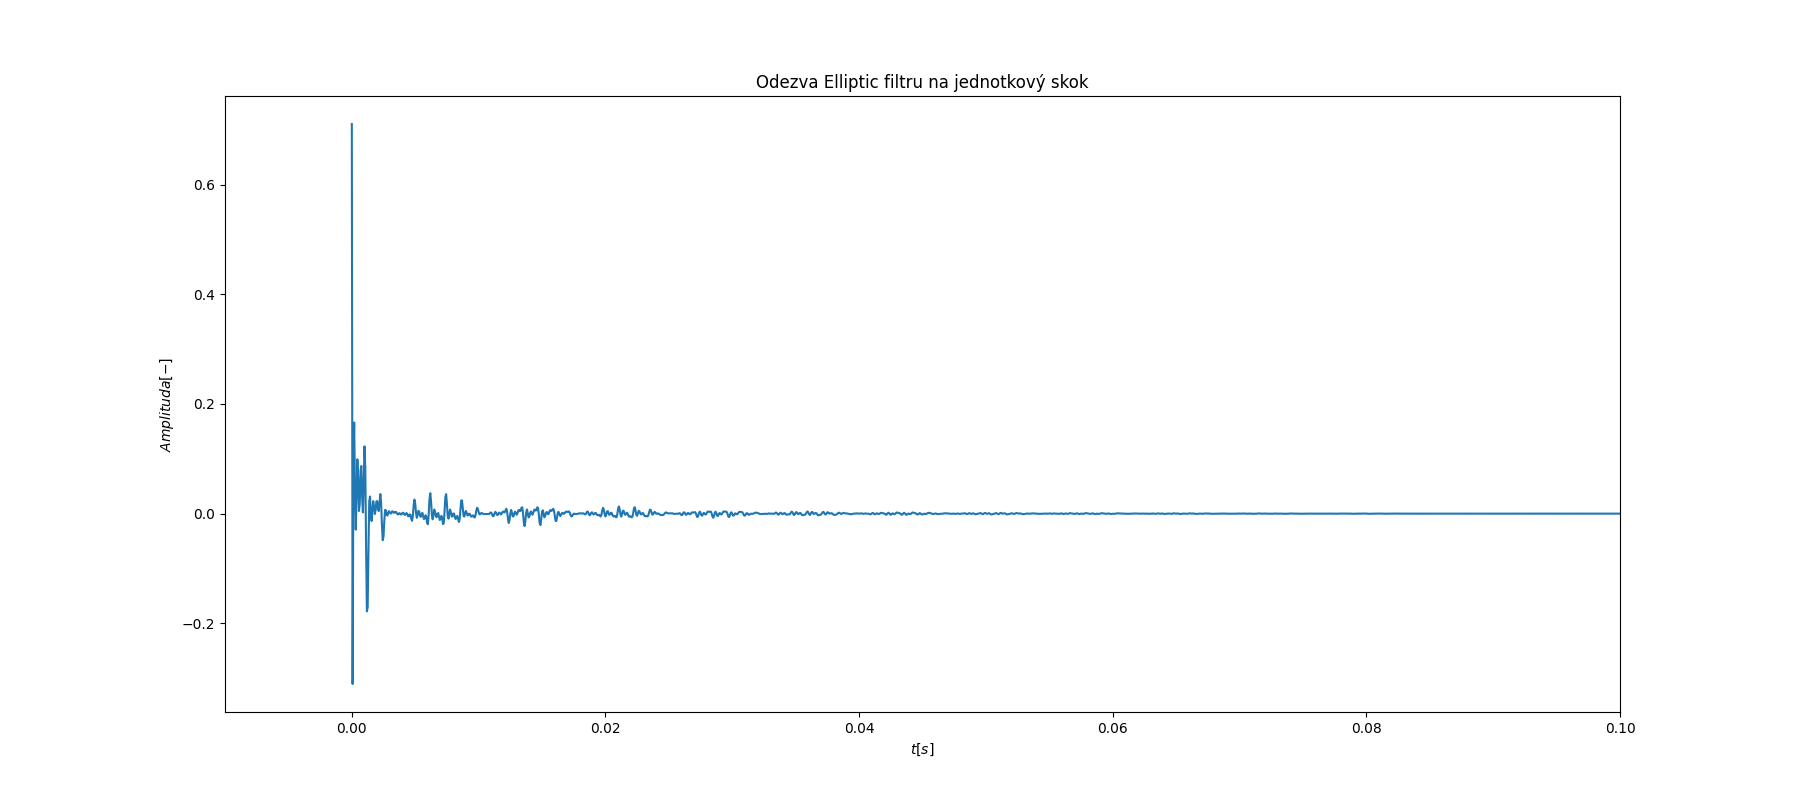
\includegraphics[scale=0.40,keepaspectratio]{Figure_22}
	\caption{Odezva na jednotkový skok spojených Elliptic filtrů}
\end{figure}

\begin{figure}[H] 
	\centering
	\includegraphics[scale=0.40,keepaspectratio]{Figure_44}
	\caption{Odezva na jednotkový skok Elliptic filtru 1}
\end{figure}

\begin{figure}[H] 
	\centering
	\includegraphics[scale=0.40,keepaspectratio]{Figure_45}
	\caption{Odezva na jednotkový skok Elliptic filtru 2}
\end{figure}

\begin{figure}[H] 
	\centering
	\includegraphics[scale=0.40,keepaspectratio]{Figure_46}
	\caption{Odezva na jednotkový skok Elliptic filtru 3}
\end{figure}

\begin{figure}[H] 
	\centering
	\includegraphics[scale=0.40,keepaspectratio]{Figure_47}
	\caption{Odezva na jednotkový skok Elliptic filtru 4}
\end{figure}


\subsubsection{Butterworth filtr}

\begin{figure}[H] 
	\centering
	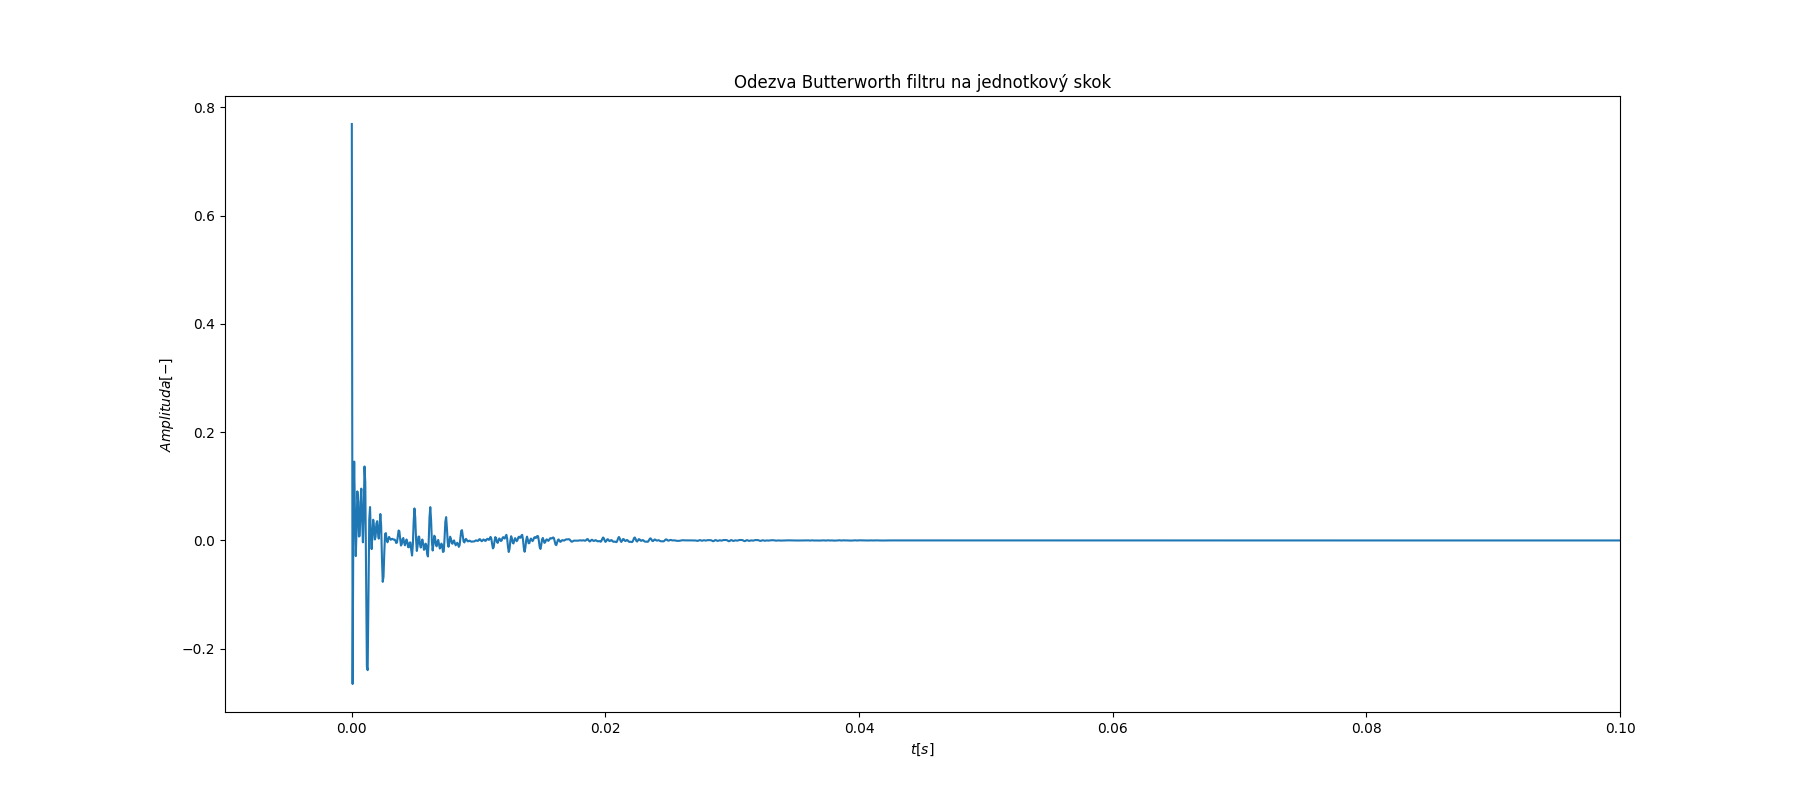
\includegraphics[scale=0.40,keepaspectratio]{Figure_24}
	\caption{Odezva na jednotkový skok spojených Butterworth filtrů}
\end{figure}

\begin{figure}[H] 
	\centering
	\includegraphics[scale=0.40,keepaspectratio]{Figure_48}
	\caption{Odezva na jednotkový skok Butterworth filtru 1}
\end{figure}

\begin{figure}[H] 
	\centering
	\includegraphics[scale=0.40,keepaspectratio]{Figure_50}
	\caption{Odezva na jednotkový skok Butterworth filtru 2}
\end{figure}

\begin{figure}[H] 
	\centering
	\includegraphics[scale=0.40,keepaspectratio]{Figure_51}
	\caption{Odezva na jednotkový skok Butterworth filtru 3}
\end{figure}

\begin{figure}[H] 
	\centering
	\includegraphics[scale=0.40,keepaspectratio]{Figure_52}
	\caption{Odezva na jednotkový skok Butterworth filtru 4}
\end{figure}
